\section{Why does MongoDB's \approachName Optimizer Avoid Collection Scan?}
\label{sec:rootcauseanalysis}
% Nevertheless, we observed that the change we made still not sufficient to always generate optimal query plans. The reasoning behind the preference bias is unknown. 
As we just saw in Section \ref{sec:evaluation}, MongoDB's \approachName optimizer doesn't choose collection scan plans, even for queries when it would run substantially faster than using an index. In this section, we take a closer look at the code of the optimizer to identify reasons for this preference bias issue in MongoDB.

A closer inspection of the query optimizer code revealed a surprising design choice:
% The simple fact is that MongoDB doesn't include collection scan in the list of candidate plans to be run in \approachName, when there is also an index scan available! 

% Michael's scratch area to copy/paste later
by default, MongoDB 4.4.0 does not include collection scan among the list of candidate plans to be run in \approachName, if an index is available to satisfy a query.  In more detail, line 1082 of \texttt{src/\-mongo/\-db/\-query/\-query\_planner.cpp} \footnote{\url{https://github.com/mongodb/mongo/blob/r4.4.0/src/mongo/db/query/query_planner.cpp\#L1082}} is the check before a collection scan is included:

\begin{verbatim}
   if (possibleToCollscan &&
      (collscanRequested || collScanRequired)) { ...
\end{verbatim}

The variable \texttt{possibleToCollscan} indicates whether a collection scan is possible (database administrators can disable collection scans or the query can include a hint that requires use of an index); \texttt{collscanRequested} indicates that an explicit query hint has specified that a collection scan should be used; and \texttt{collScanRequired} is true only if there is no matching index.  In other words, if a matching index exists, a collection scan must be explicitly requested for MongoDB to consider it.  If the collection scan isn't tasking part, it can't win the race.

\begin{figure}[htb]
    \centering
%    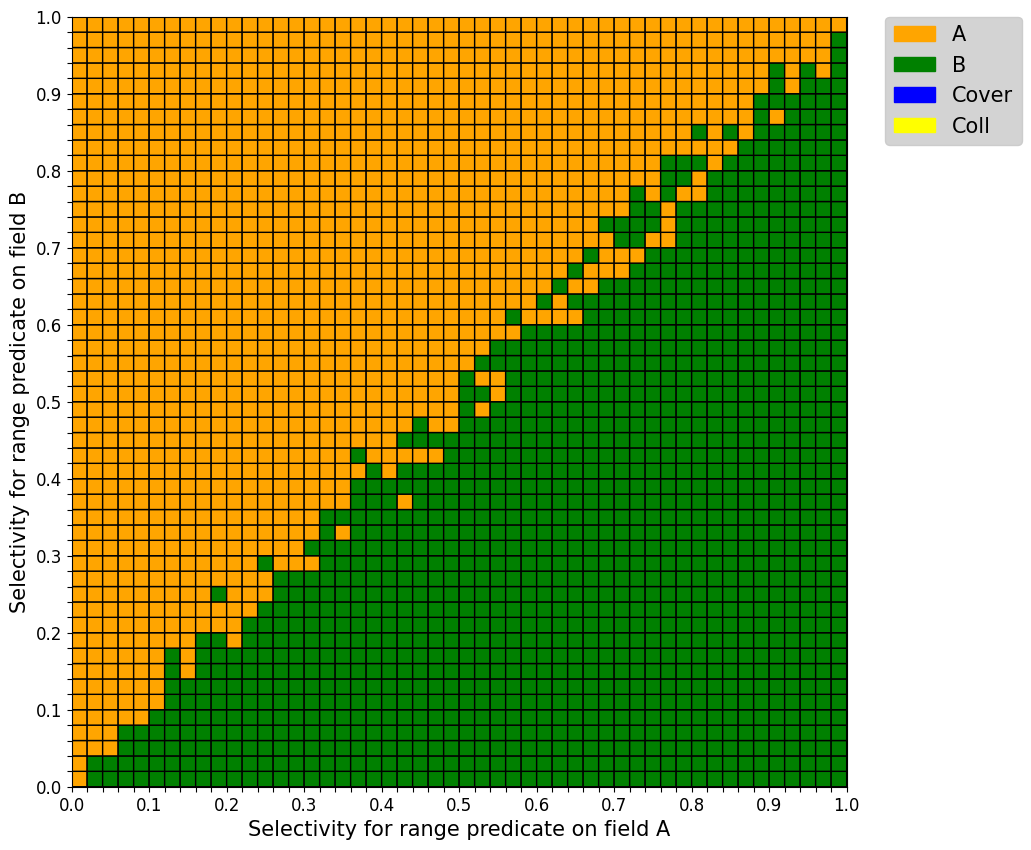
\includegraphics[width=0.9\columnwidth]{images/results-without-covering-index/mongo-with-coll/comprehensive_mongo_choice.png}
    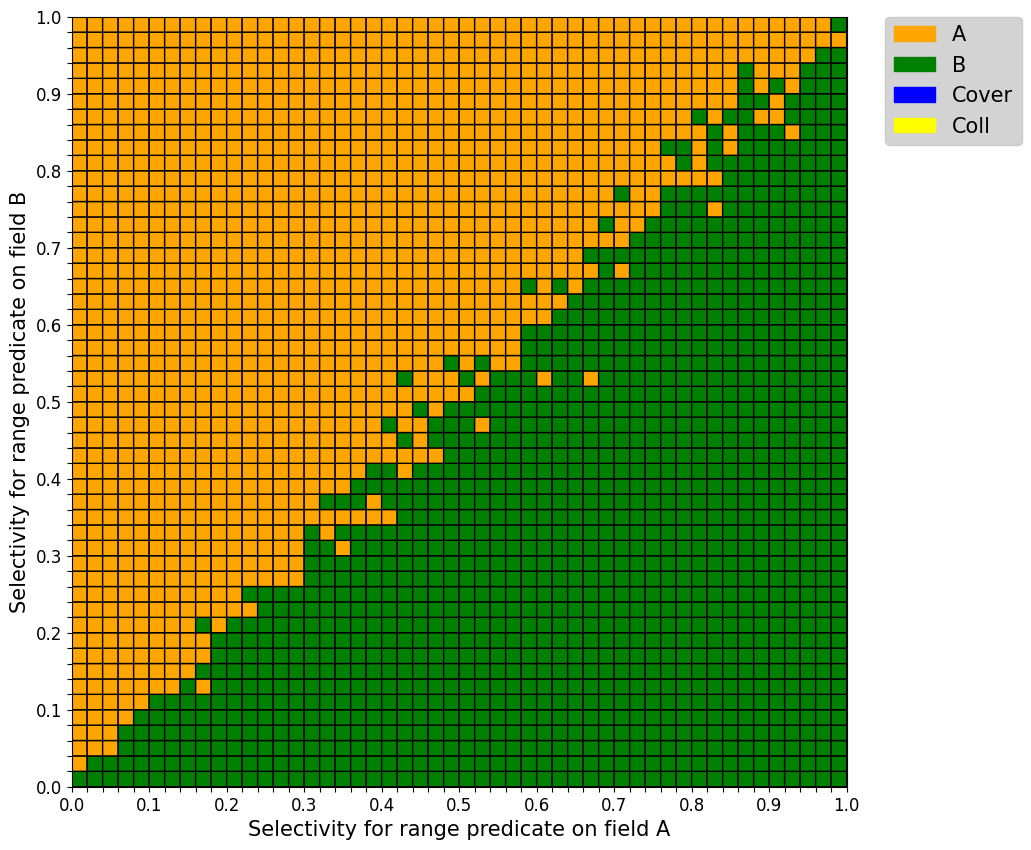
\includegraphics[width=0.9\columnwidth]{images/results-without-covering-index/mongo-with-coll/72169da5f0334b6c8f1c9de4ed9b7248_mongo_choice.png}
    \caption{Chosen plans by MongoDB+COLLSCAN.}
    \label{fig:mongo-v1-bothindexed-choices}
\end{figure}

\subsection{Forcing consideration of the collection scan}
However, is this all there is to the issue? We modified the source code to produce a variant we call MongoDB+COLLSCAN that simply always adds a COLLSCAN plan to the set of candidate plans which MongoDB's \approachName optimizer tries out. We repeated our experiments with this variant dbms, and we did not see substantial differences in the chosen plans, from unmodified MongoDB 4.4.0 (cf. Figure~\ref{fig:mongo-v1-bothindexed-choices}). That is, even when COLLSCAN is considered in the \approachName race, it does not win, even for queries where the collection scan plan runs substantially faster than an alternative plan with index scan.



\begin{figure*}[t]
%\newlength\plotheight%
\setlength\plotheight{\heightof{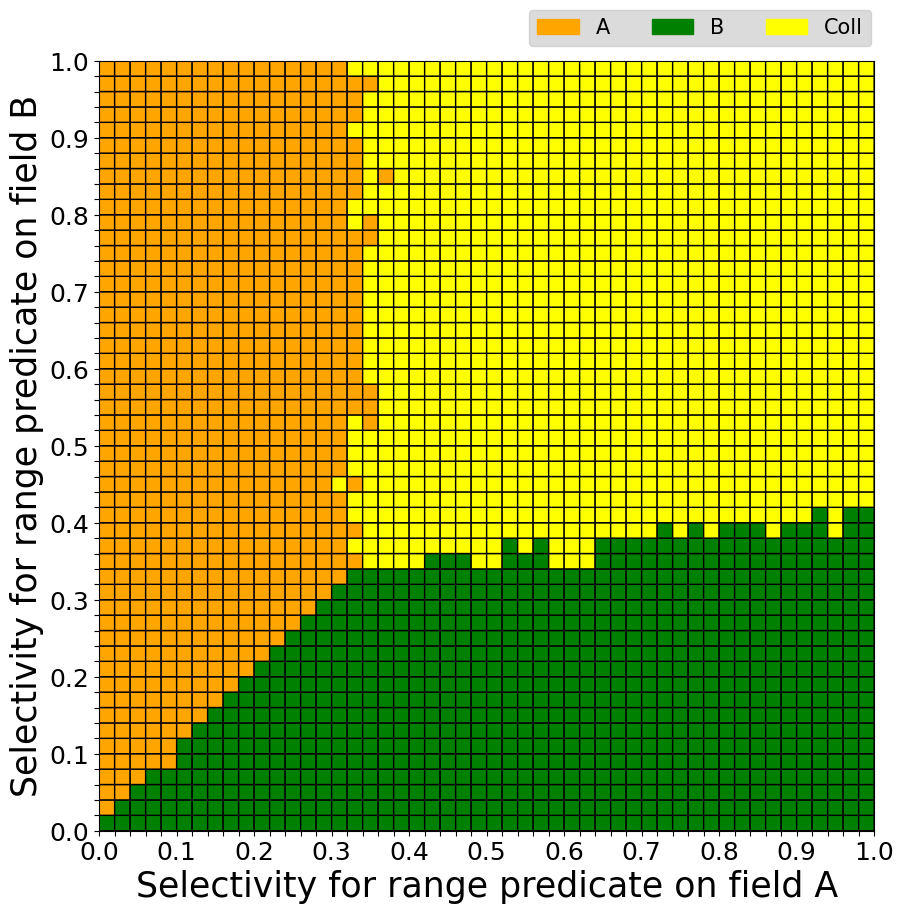
\includegraphics[width=0.3\textwidth]{images/results-without-covering-index/mongo-with-coll-with-fix/comprehensive_practical_winner.png}}}
    \centering
    \subfigure[Plans chosen by MongoDB\_MOD.]{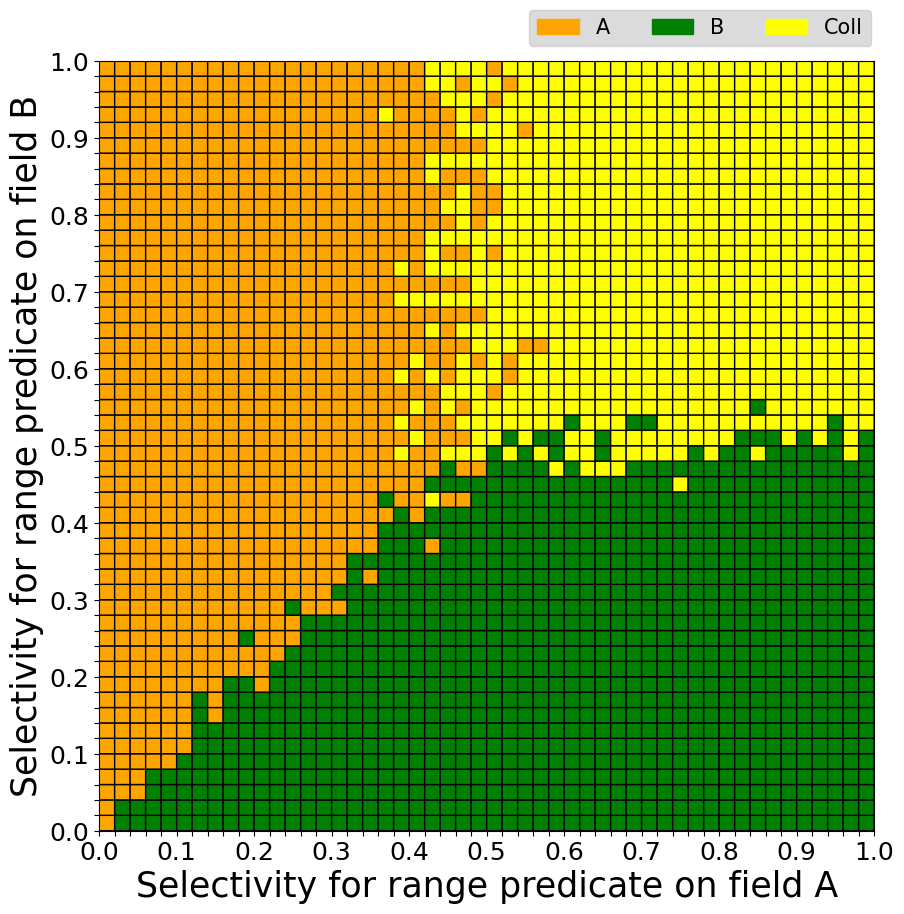
\includegraphics[height=\plotheight]{images/results-without-covering-index/mongo-with-coll-with-fix/comprehensive_mongo_choice.png}\label{fig:mongo-v2-choices}} 
    \quad
%    \begin{subfigure}%[b]{0.3\textwidth}
%         \centering
%          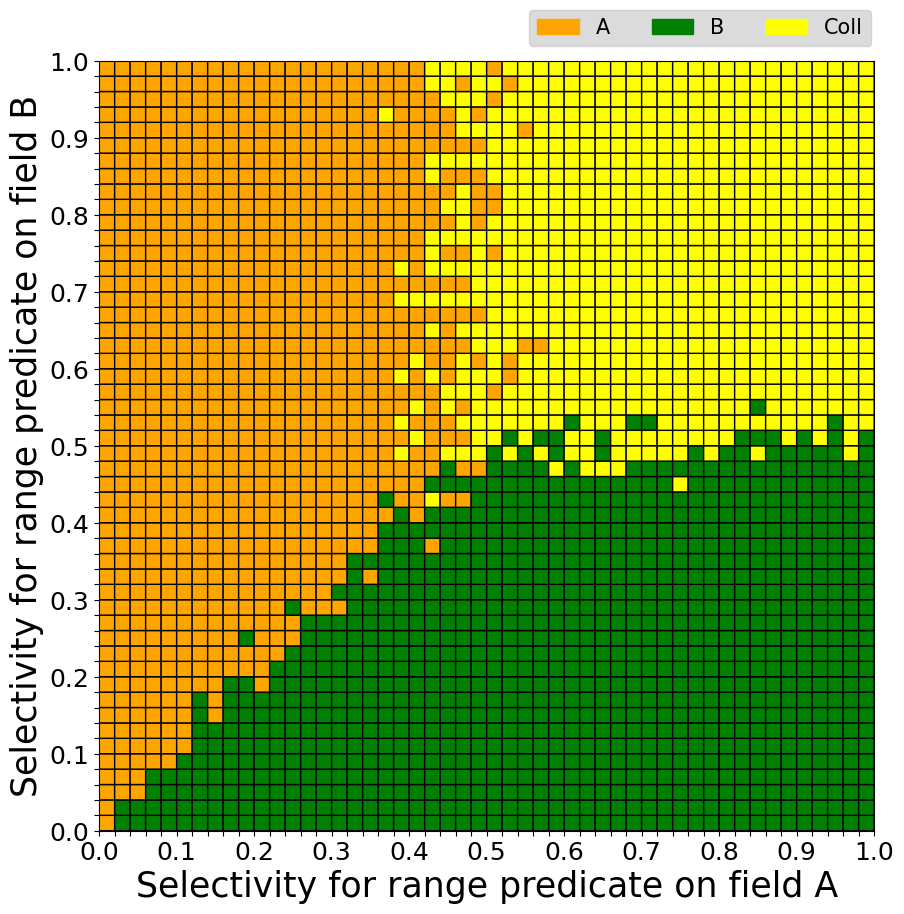
\includegraphics[width=0.3\textwidth]{images/results-without-covering-index/mongo-with-coll-with-fix/comprehensive_mongo_choice.png}
%         \caption{Plans chosen by MongoDB\_MOD.}
%         \label{fig:mongo-choice-v2}
%    \end{subfigure}%
    \subfigure[Optimal Plan Choices.]{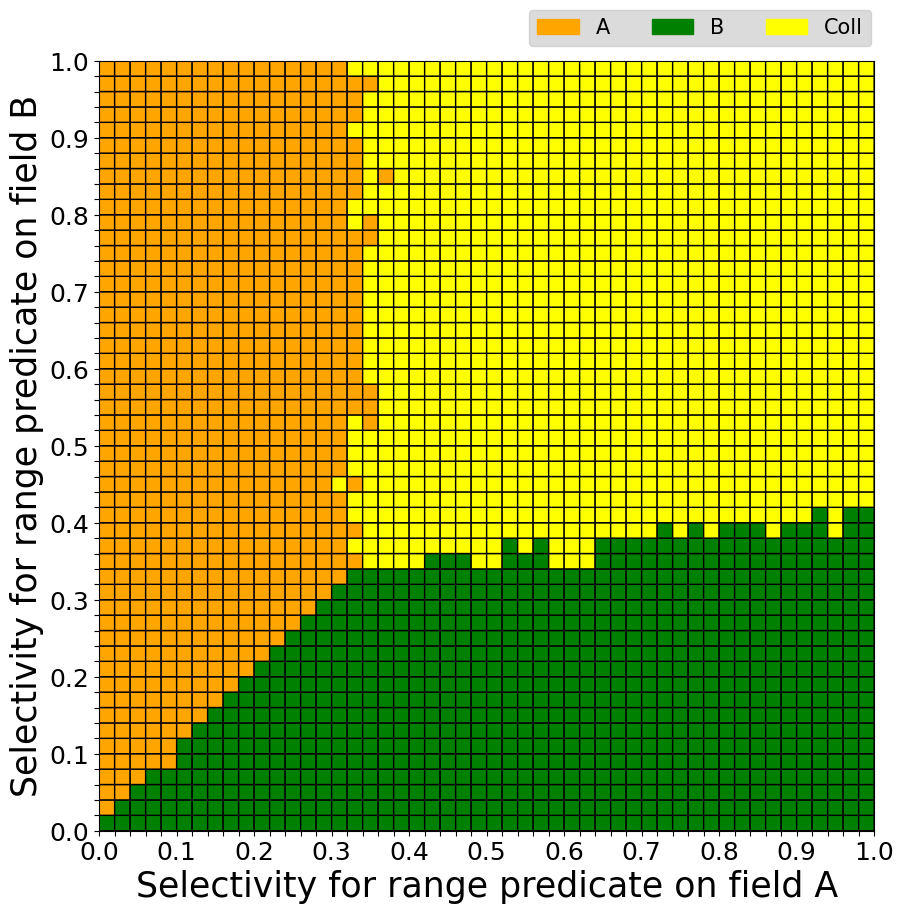
\includegraphics[height=\plotheight]{images/results-without-covering-index/mongo-with-coll-with-fix/comprehensive_practical_winner.png}\label{fig:mongo-v2-optimal}} 
    \quad
%    \begin{subfigure}%[b]%{0.3\textwidth}
%         \centering
%         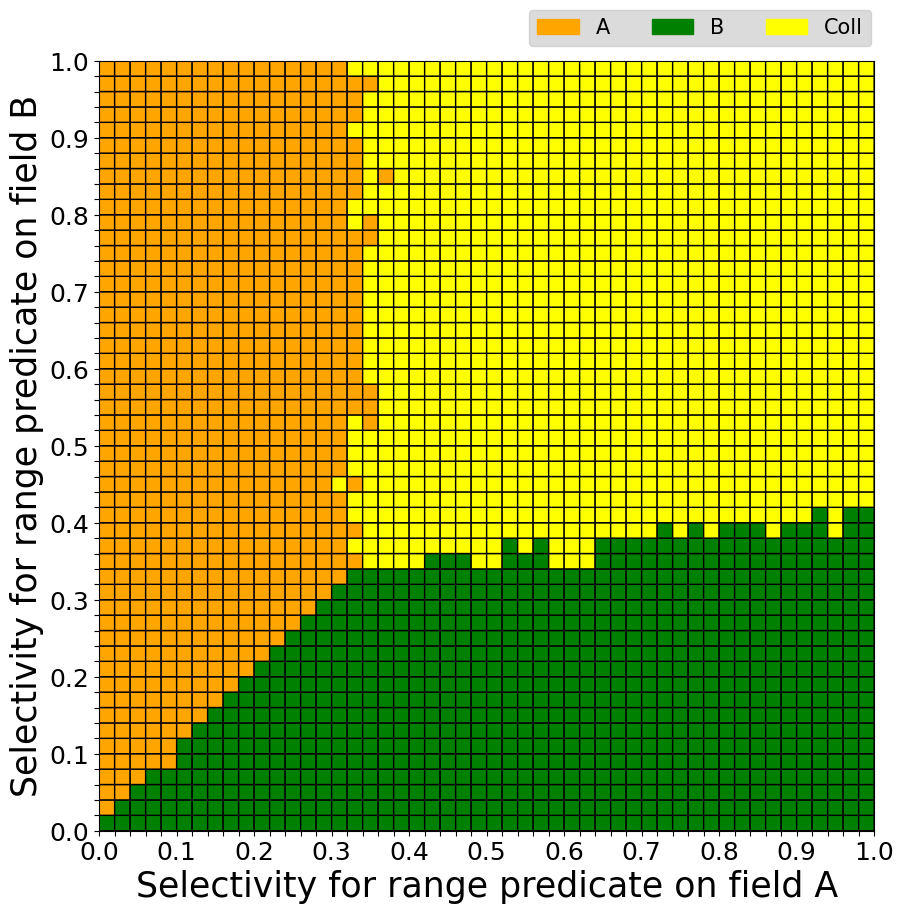
\includegraphics[width=0.3\textwidth]{images/results-without-covering-index/mongo-with-coll-with-fix/comprehensive_practical_winner.png}
%         \caption{Optimal Plan Choices.}
%         \label{fig:mongo-with-coll-v2}
%    \end{subfigure}%
    \subfigure[Performance Impact of MongoDB\_MOD's choices.]%: Accuracy = 85.12\%, Performance diff = 1.02\%.]
    {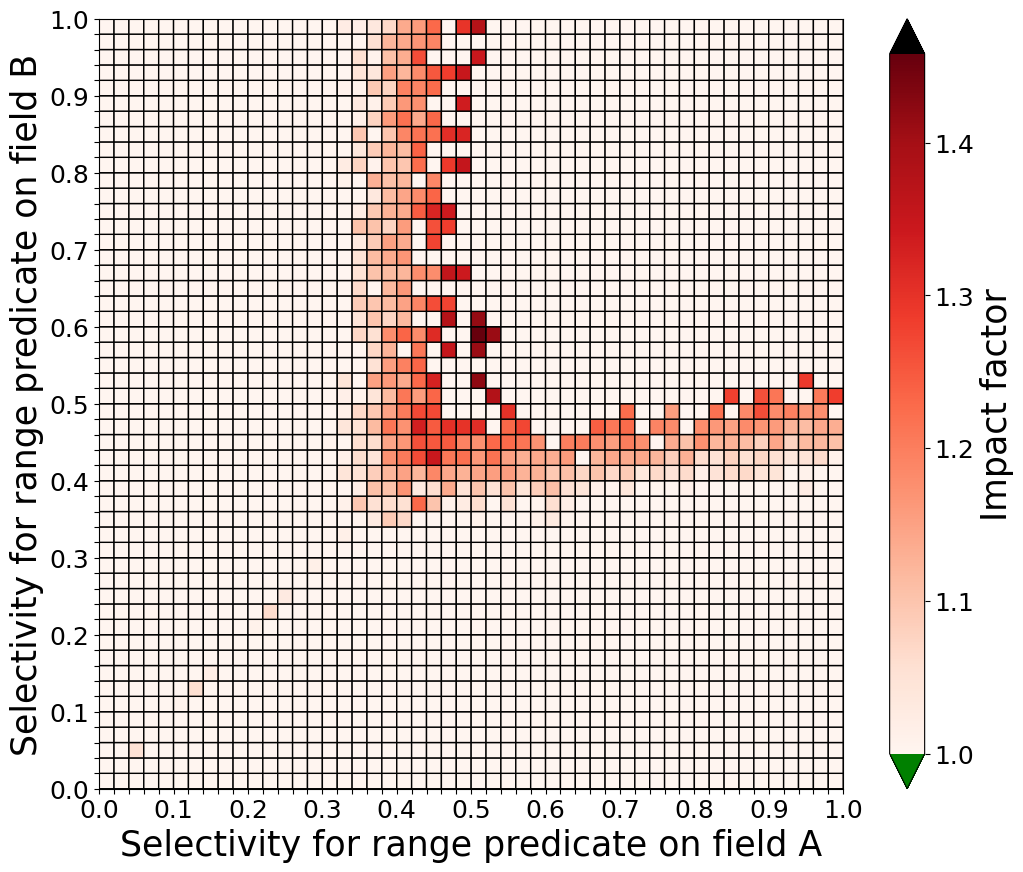
\includegraphics[height=\plotheight]{images/results-without-covering-index/mongo-with-coll-with-fix/comprehensive_summary_accuracy=85.12_impact_factor=1.01983.png}\label{fig:mongo-v2-perfimpact}}
%    \begin{subfigure}%[b]%{0.3\textwidth}
%         \centering
%         \includegraphics[width=0.28\textwidth]{images/results-without-covering-index/mongo-with-coll-with-fix/comprehensive_summary_accuracy=85.12_overall_percentage_change=2.09.png}
%        \caption{Performance Impact: Accuracy = 85\%, Performance diff = 2.09\%.}
%         \label{fig:mongo-with-fix-v2}
%    \end{subfigure}%
     \vspace*{-0.5\baselineskip}
     \caption{Effectiveness of modified \approachName query pptimizer of MongoDB\_MOD (dual index scenario).}
     \label{fig:mongo-v2-evaluation}
\end{figure*}

%%%%%%%%%%%%%%%%%%%%%%%%%%%%%%%%%%%%%%%%%%
%     impact on the single index case    %
% [UR: I think we concentrate on dual-index and covering index in this part] %
%%%%%%%%%%%%%%%%%%%%%%%%%%%%%%%%%%%%%%%%%%
%
%\begin{figure*}[t]
%\newlength\plotheight%
%\setlength\plotheight{\heightof{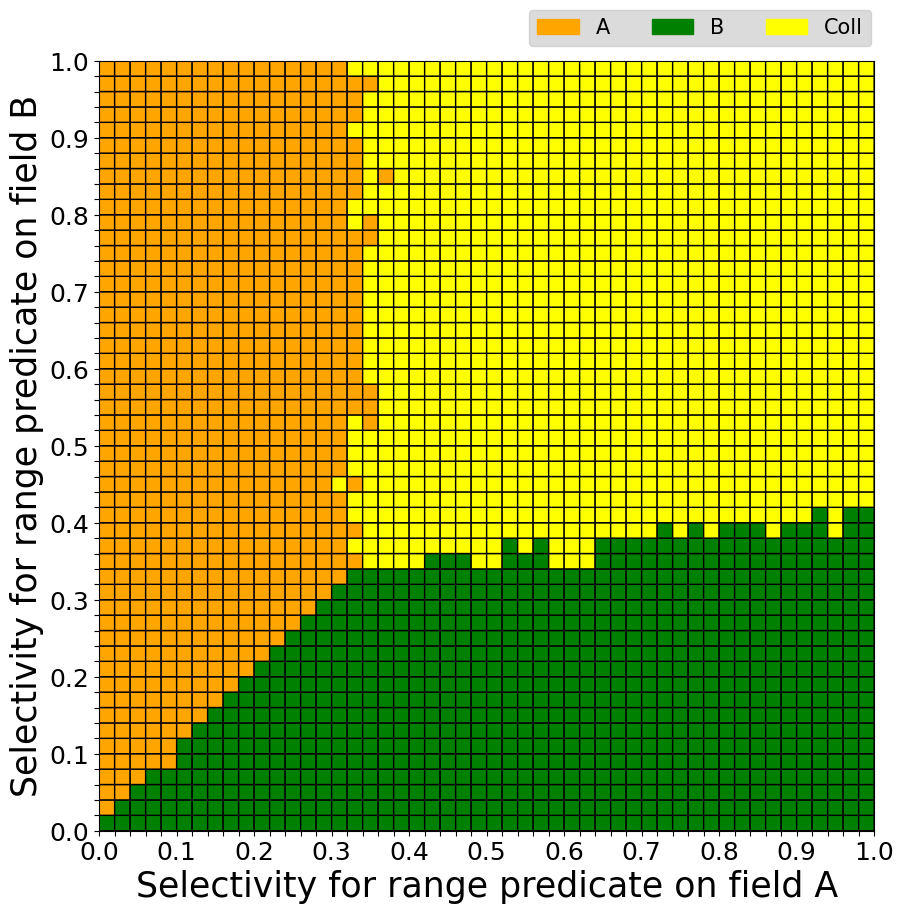
\includegraphics[width=0.3\textwidth]{images/results-without-covering-index/mongo-with-coll-with-fix/comprehensive_practical_winner.png}}}
%    \centering
%    \subfigure[Plans chosen by MongoDB\_MOD.]{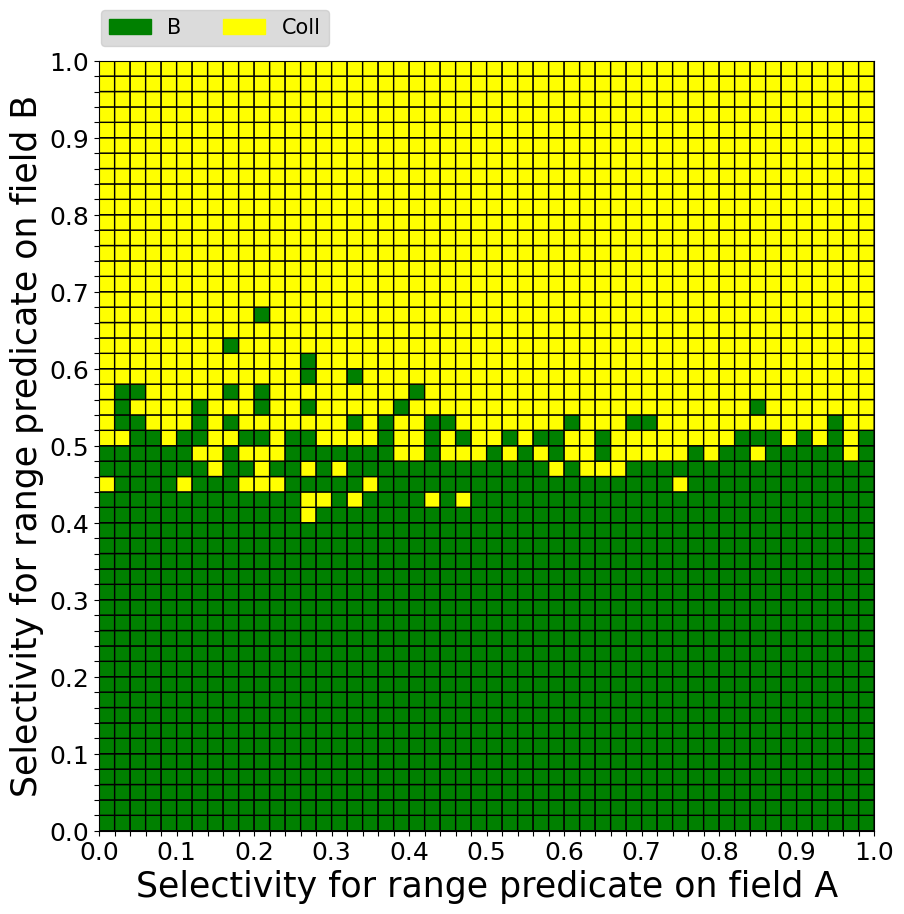
\includegraphics[height=\plotheight]{images/mongo-mod-effect/single-index/comprehensive_mongo_choice.png}\label{fig:mongo-v2-choices-single}} 
%    \quad
%    \begin{subfigure}%[b]{0.3\textwidth}
%         \centering
%          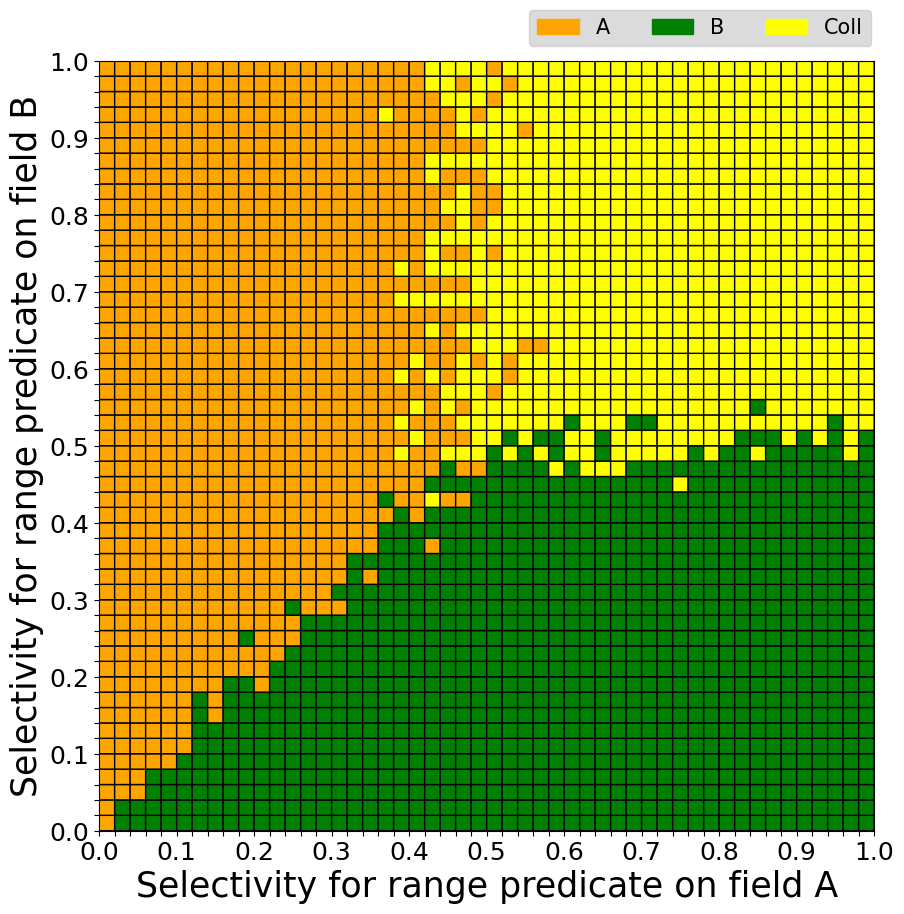
\includegraphics[width=0.3\textwidth]{images/results-without-covering-index/mongo-with-coll-with-fix/comprehensive_mongo_choice.png}
%         \caption{Plans chosen by MongoDB\_MOD.}
%         \label{fig:mongo-choice-v2}
%    \end{subfigure}%
%    \subfigure[Optimal Plan Choices.]{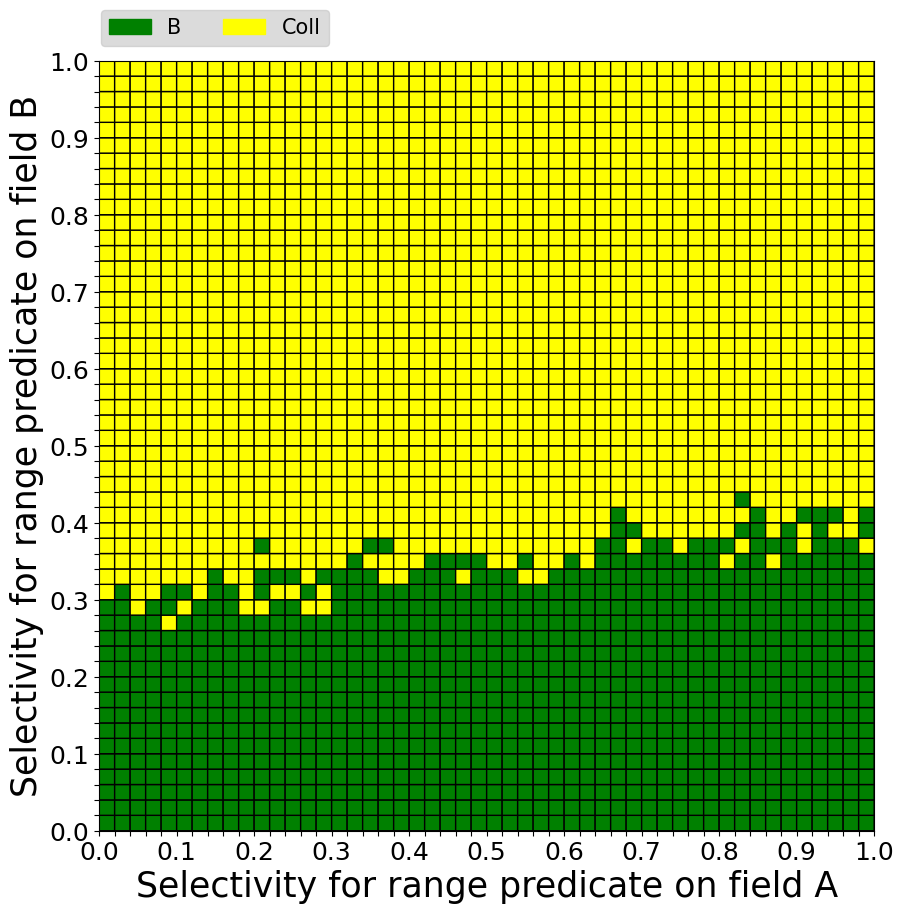
\includegraphics[height=\plotheight]{images/mongo-mod-effect/single-index/comprehensive_practical_winner.png}\label{fig:mongo-v2-optimal-single}} 
%    \quad
%    \begin{subfigure}%[b]%{0.3\textwidth}
%         \centering
%         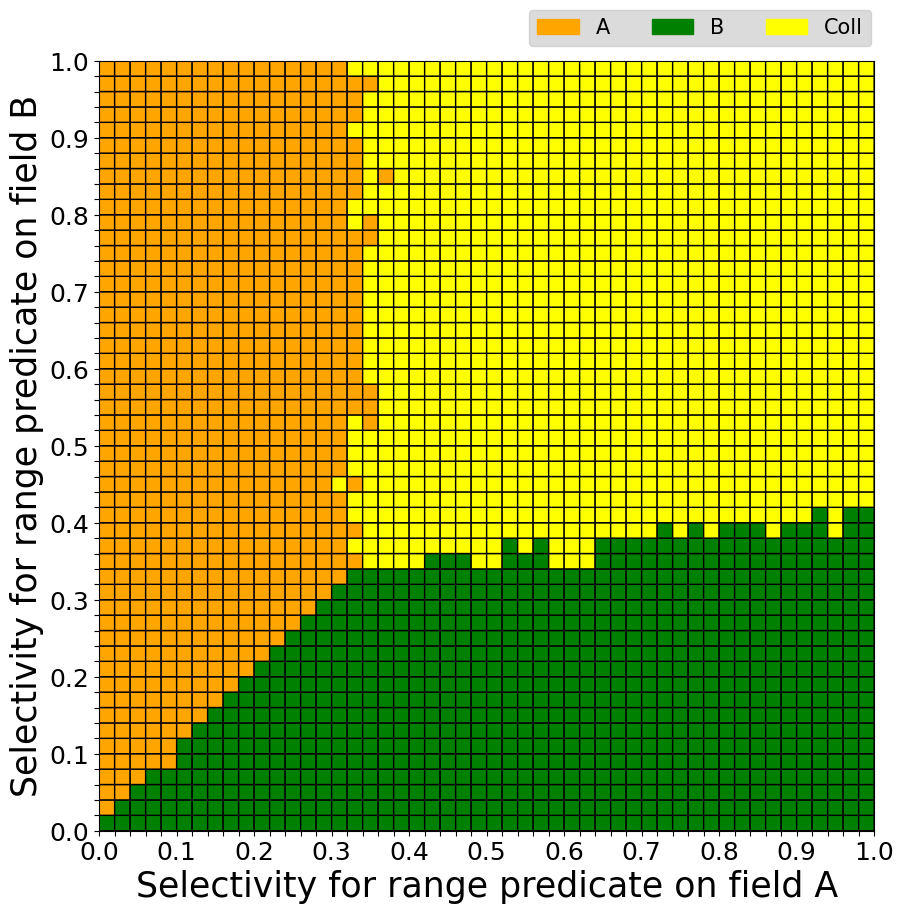
\includegraphics[width=0.3\textwidth]{images/results-without-covering-index/mongo-with-coll-with-fix/comprehensive_practical_winner.png}
%         \caption{Optimal Plan Choices.}
%         \label{fig:mongo-with-coll-v2}
%    \end{subfigure}%
%    \subfigure[Performance Impact of MongoDB\_MOD's choices.]%: Accuracy = 85.12\%, Performance diff = 1.02\%.]
%    {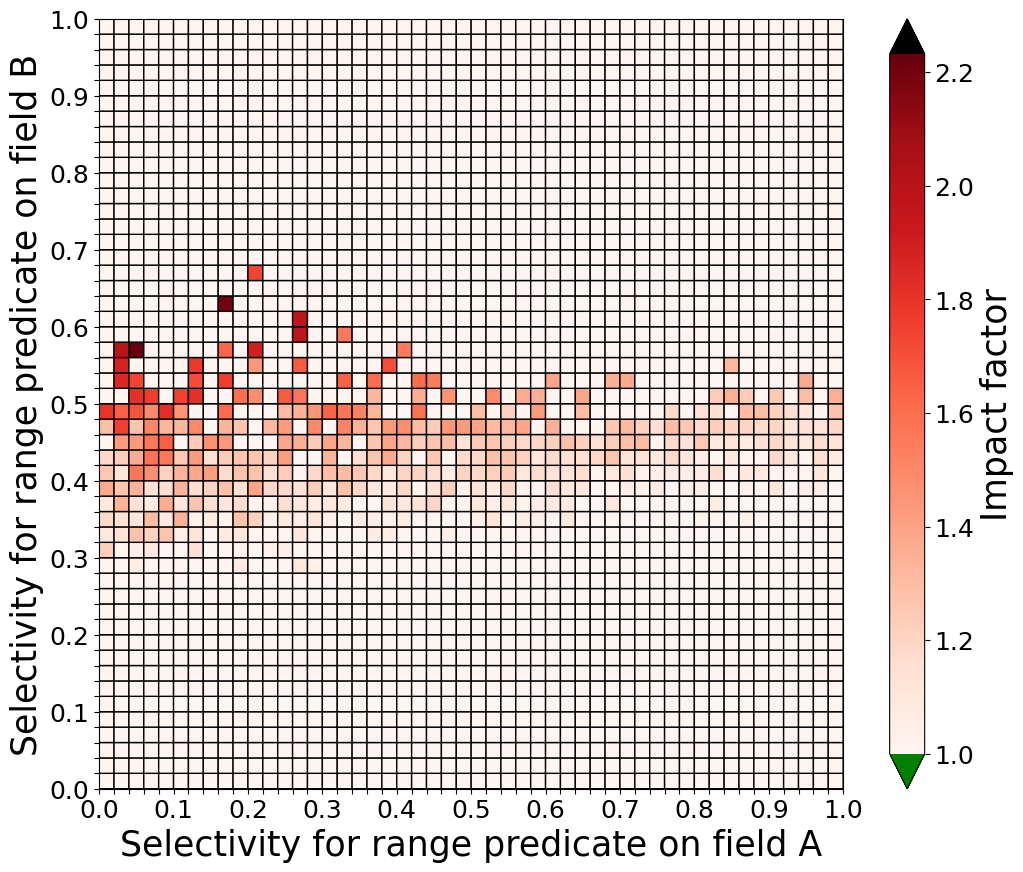
\includegraphics[height=\plotheight]{images/mongo-mod-effect/single-index/comprehensive_summary_accuracy=84.68_impact_factor=1.03932.png}\label{fig:mongo-v2-perfimpact-single}}
%    \begin{subfigure}%[b]%{0.3\textwidth}
%         \centering
%         \includegraphics[width=0.28\textwidth]{images/results-without-covering-index/mongo-with-coll-with-fix/comprehensive_summary_accuracy=85.12_overall_percentage_change=2.09.png}
%        \caption{Performance Impact: Accuracy = 85\%, Performance diff = 2.09\%.}
%         \label{fig:mongo-with-fix-v2}
%    \end{subfigure}%
%     \vspace*{-0.5\baselineskip}
%     \caption{Effectiveness modified \approachName query optimizer of MongoDB\_MOD (single index scenario).}
%     \label{fig:mongo-v2-evaluation-single}
%\end{figure*}

%%%%%%%%%%%%%%%%%%%%%%%%%%%%%%%%%%%%%%%%%%%%
%     impact on the covering index case    % 
%%%%%%%%%%%%%%%%%%%%%%%%%%%%%%%%%%%%%%%%%%%%
\begin{figure*}[t]
%\newlength\plotheight%
\setlength\plotheight{\heightof{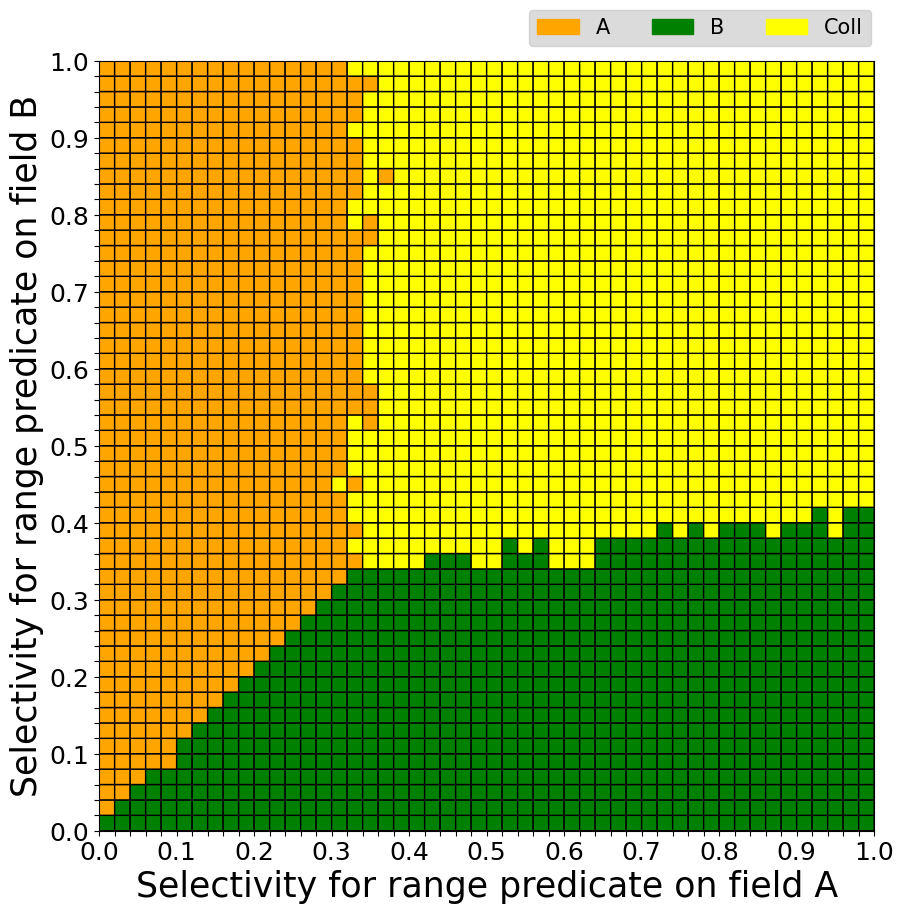
\includegraphics[width=0.3\textwidth]{images/results-without-covering-index/mongo-with-coll-with-fix/comprehensive_practical_winner.png}}}
    \centering
    \subfigure[Plans chosen by MongoDB\_MOD.]%. \textbf{Covering Index}]
    {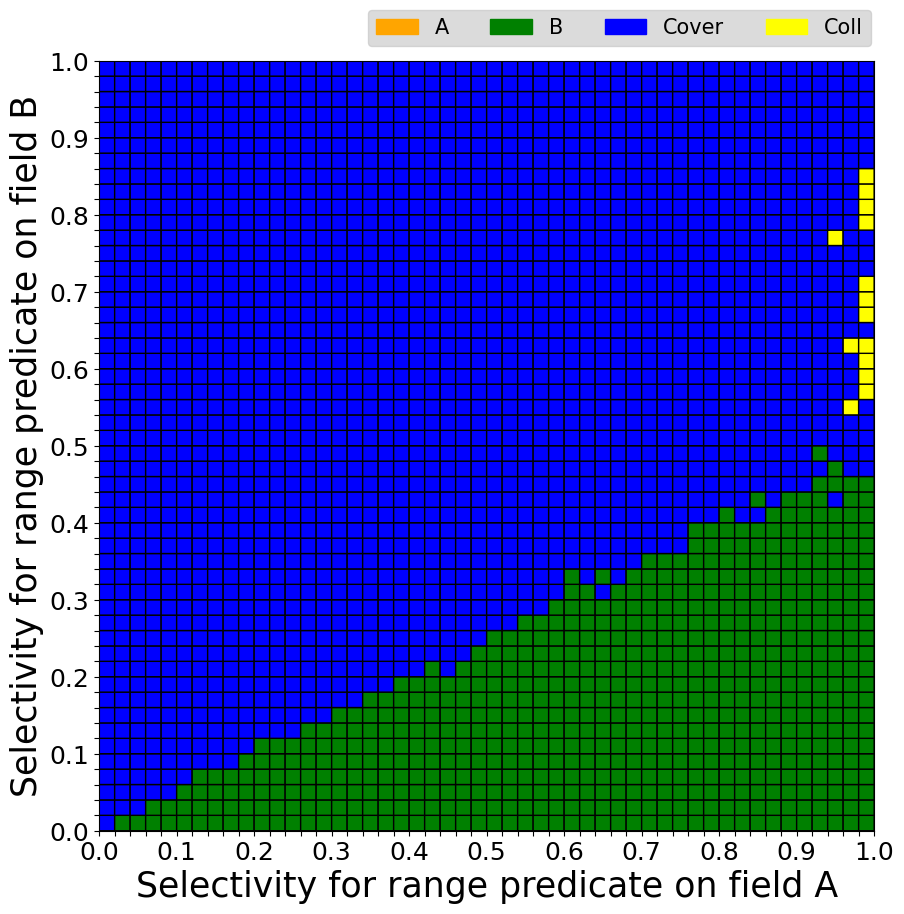
\includegraphics[height=\plotheight]{images/mongo-mod-effect/covering-index/comprehensive_mongo_choice.png}\label{fig:mongo-v2-coveringindex-choices}} 
    \quad
%    \subfigure[Optimal Plan Choices.]{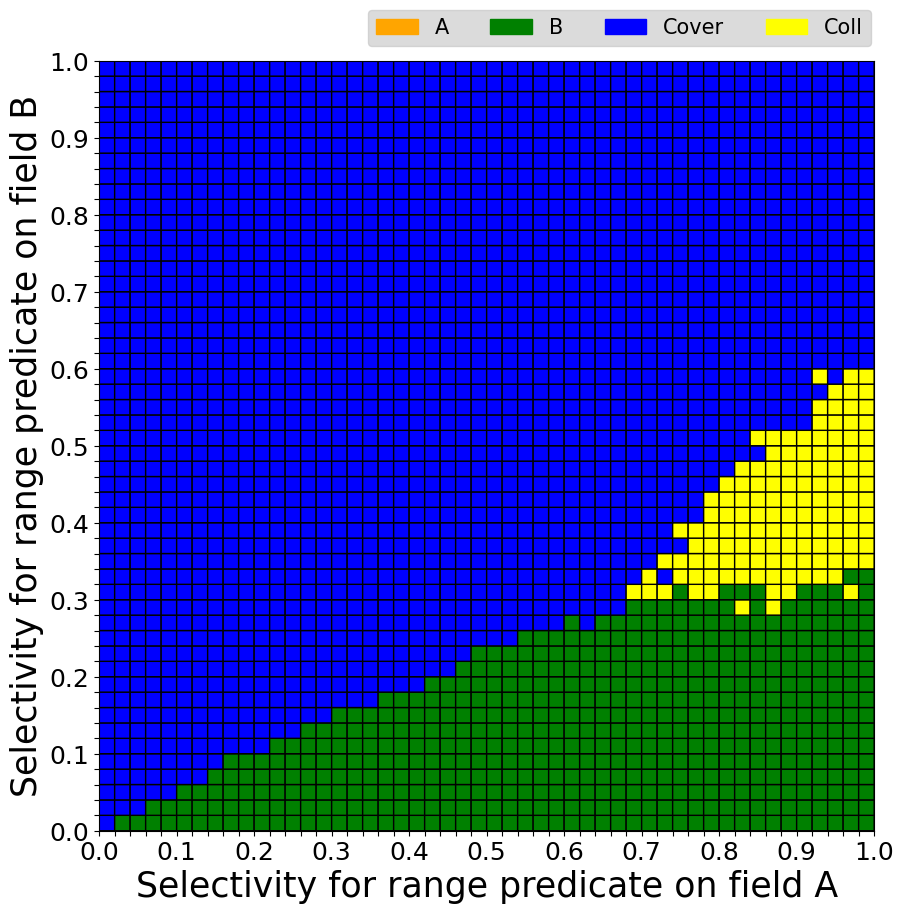
\includegraphics[height=\plotheight]{images/results-with-covering-index/mongo-original/comprehensive_practical_winner.png}\label{fig:mongo-v2-coveringindex-optimal}} 
    \subfigure[Optimal Plan Choices.]{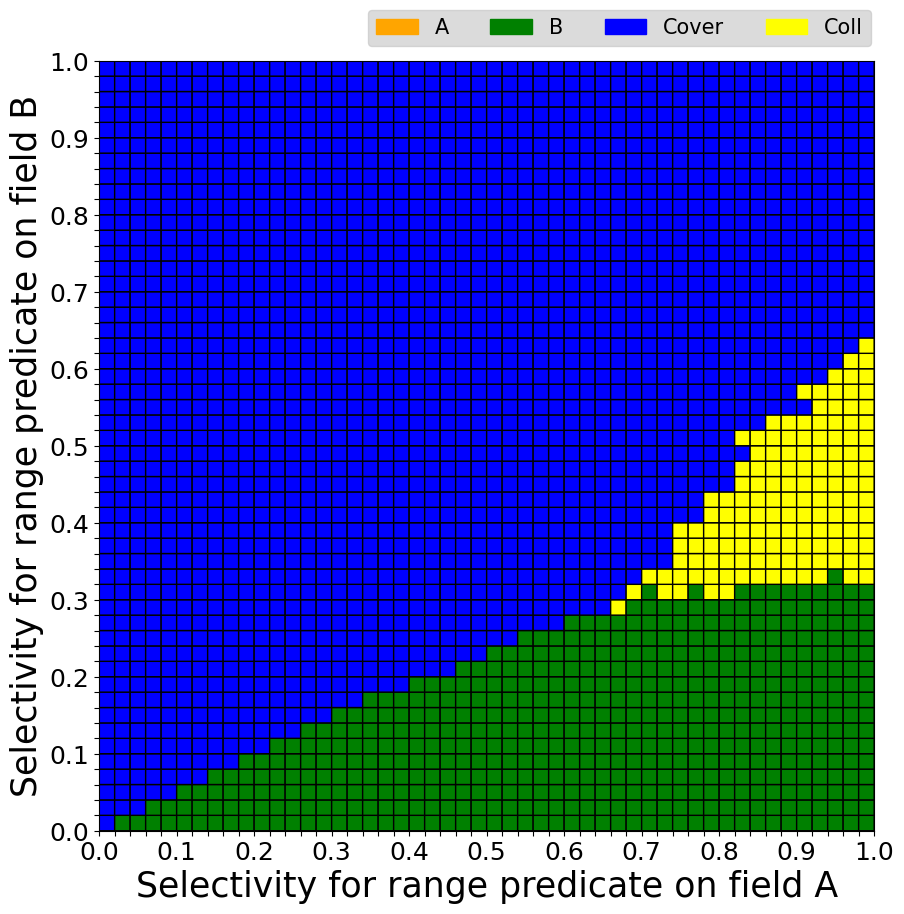
\includegraphics[height=\plotheight]{images/mongo-mod-effect/covering-index/comprehensive_practical_winner.png}\label{fig:mongo-v2-coveringindex-optimal}} 
    \quad
    \subfigure[Performance Impact of MongoDB\_MOD's choices.]%: Accuracy = 85.12\%, Performance diff = 1.02\%.]
    {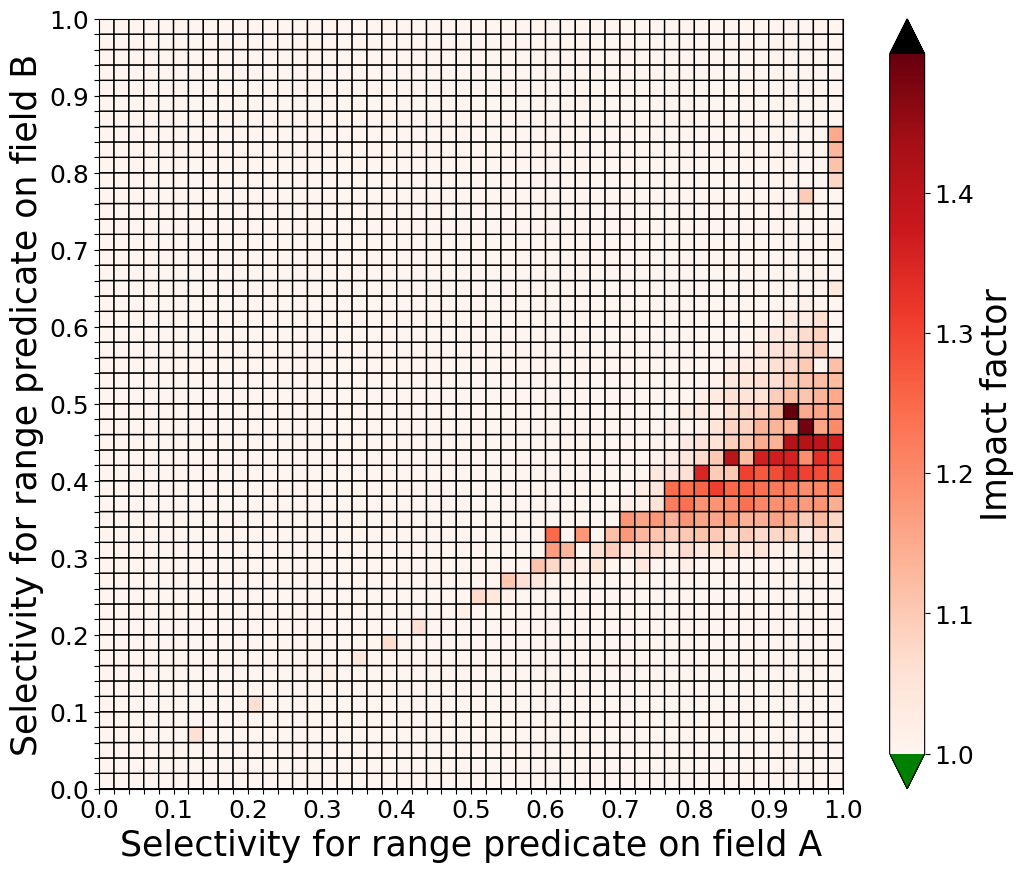
\includegraphics[height=\plotheight]{images/mongo-mod-effect/covering-index/comprehensive_summary_accuracy=91.24_impact_factor=1.01018.png}\label{fig:mongo-v2-coveringindex-perfimpact}}
     \vspace*{-0.5\baselineskip}
     \caption{Effectiveness of modified \approachName query optimizer of MongoDB\_MOD (covering index scenario).}
     \label{fig:mongo-v2-evaluation-coveringindex}
\end{figure*}



\vspace*{-0.5\baselineskip}
\subsection{Overrated Index Scan}
To explore further the cause of the preference bias that over-rates the index scan compared to collection scan, we looked in detail at the query execution log showing the activity of MongoDB+COLLSCAN during the optimization race for a query with selectivity 0.95 in each attribute. In the visualizations above, we see that for this query collection scan is clearly superior, but the optimizer chooses to use an index. As we mentioned in Section~\ref{sec:background}, the \approachName approach assigns a score to summarize the performance of each query plan at the end of the race (and then the query plan with the highest score will be chosen). The formula considers the $productivity$ of each query plan, where productivity is based on the ratio between result documents produced and the work units performed during the race. Note that these work units represent logical costs, not actual measured runtimes.

As it turns out, when determining the workUnit of an index scan, the MongoDB implementation of the \approachName approach ignores the cost of fetching index documents; the optimizer in MongoDB 4.4.0 treats the index retrieving work and the document retrieving work together as a single unit of work (i.e. the same amount of work required by a collection scan looking at the same number of documents). Therefore, the workunit is under-counted for the index scan and so the productivity of an index scan is overrated. This implementation detail in MongoDB's query optimizer code hides the true advantage of a collection scan in many cases.  We suggest that it would be appropriate for MongoDB to adjust the way workunit is measured in the race, to correct this.

\subsection{Adjusting productivity score of index scan}
We showed above that the optimizer ascribes too much productivity to the index scan, because it treats as 1~workunit, the combination of retrieving the index entry, and retrieving the document the index points to. So we made another small modification to the optimizer code. When the plan contains a FETCH (that is, when there is a lookup through the index) we simply halved the productivity score calculated. This is overly simplistic for complex query plans, but its a reasonable shortcut for the simple queries in these experiments. We call the variant system with forced consideration of COLLSCAN, and also with the adjusted productivity score as described, MongoDB\_MOD.  This system is evaluated for the physical design with uniform data distribution and two indices, in Figures~\ref{fig:mongo-v2-choices}--\ref{fig:mongo-v2-perfimpact}. We see that, while the modified score is not a perfect adjustment, it gets the right decision in many of the queries, and the chosen plan is never worse by much than the best possible. 
%New text by Alan
We remark that, in theory, the optimal plan choice ought to be exactly the same for this system as for unmodified MongoDB 4.4.0 since the only change is in the optimiser rather than in query plan execution (that is, Fig~\ref{fig:mongo-v2-optimal} should be the same as Fig~\ref{fig:mongo-bothindexed-optimal}. This is not exactly the case, because each figure is produced from measurements of the running time of the plans, and there is some experimental variation from run to run; however the differences are only occasional cells near the region boundary, where two plans have almost the same cost, so which is fastest (by a tiny amount) can vary between runs.

The overall accuracy of the query optimizer of this modified version of MongoDB is now 85\% (up from just 52\% measured in Section~\ref{sec:evaluation_bothindexed}), with an average performance impact of the remaining sub-optimal plan choices of just 2\%. 


The suggested adjustment of the score of index scans also helps in the scenario with a physical design including covering indexes, as shown in Figure~\ref{fig:mongo-v2-evaluation-coveringindex}. If we compare the plan choices of the modified \approachName optimizer in Figure~\ref{fig:mongo-v2-coveringindex-choices} with the ones done by the original MongoDB 4.4.0's optimizer in Figure~\ref{fig:mongo-coveringindex-choices}, we not only see collection scans sometimes being chosen, but also note the much broader use of the covering index which resembles much closer the optimal case (the few variations near the region boundaries between the optimal cases between Figures~\ref{fig:mongo-v2-coveringindex-optimal} and \ref{fig:mongo-coveringindex-optimal} are due to slight variations in the runtimes between experiments). % SURE? [ur]
Consequently, the remaining sub-optimal plan choices by \approachName have a much reduced performance impact (cf. Figure~\ref{fig:mongo-v2-coveringindex-perfimpact}).
The overall accuracy of the modified query optimizer is now 91\%, with an average performance impact of just 1\%. 


\subsection{Discussion}
We have shown that the coding in MongoDB's \approachName query optimization has a systematic preference bias that can lead to poor choice of execution plan. The outcomes can be improved by forcing consideration of COLLSCAN in the race, and adjusting the productivity score to recognize the extra work done 
%in an index scan 
when both index lookup and then document lookup happen. Further work is needed to find more sophisticated ways to score productivity, that will deal with complicated plans with index lookup on some but not all steps. 
%(and so we need an adjustment that is more nuanced than simply halving the score).

We know that the scale of our workload 
is considerably smaller than common in real-world settings; we only measured cases where the indices all fit in memory. 
In reality, companies often have Terabytes of data
stored in MongoDB, and they have more substantial
index structures. This would significantly magnify the 
true costs of the index scan and thus dramatically 
increase the negative impact of the preference bias 
from neglecting the cost of fetching index entries. Therefore, 
in such cases, we expect that the preference bias becomes a 
much more serious issue. 

We ran earlier experiments on MongoDB 4.0.12, and we found another mistake in the code that ran the race. The count of records retrieved for the collection scan was initialised at -1 rather than as 0. This led to the collection scan always retrieving one fewer record when the race concluded. This bug has now been fixed in MongoDB 4.4.0 which we measure in this paper.




%\subsection{Query Performance Impact}
%In this section, we first illustrate the experiment results of identifying the optimal query plans through a visualization.
%We quantify the impact of the performance bias issue and  present the results through a heatmap. Through experiments we determine the accuracy of the query optimizer is only 69.29\%. Besides that, the optimal query plan is up to 86.83\% faster than MongoDB's choice. We demonstrate that the overall performance of the MongoDB query optimizer can be improved by 10.96\% if MongoDB adopt the optimal query plans. We then examine various database designs by repeating  the experiment on different dataset with various kinds of distribution to further explore the impact of this issue.We find that the distribution of the dataset does not influence MongoDB's query plan decisions. 

%\subsubsection{Visualize Optimal Query Plans}
%\begin{table}[h]
%\begin{tabular}{lllll}
%\toprule
%Case Number & Distribution of A & Distribution of B & Index on A & Index on B \\ 
%\midrule
%1           & Uniform           & Uniform           & True       & True    \\   \bottomrule
%\end{tabular}
%\caption{The database design of case 1}
%\label{tbl:c1}
%\end{table}

%Figure \ref{fig:linearv2} plots query plans chosen by MongoDB V2, while figure \ref{fig:linearreal} shows all optimal candidates MongoDB expected to  choose. Table \ref{tbl:c1} describes the physical design of this experiment. Field A and field B both have uniform distribution and we create an index on each field. The experiment result is surprisingly, we should see that the current implementation of \approachName make inappropriate choices in around one-third of  the cases. Through comparison, we found that the rate of a sub-optimal query plan been picked is 30.21\%.
%Note that the top right corner of figure \ref{fig:linearreal} is painted with yellow, it verify the theoretically analysis we made in section  \ref{sec:v1fail}. That is, for the query with high selectivty on both range predicates, the performance of a collection scan overtakes that of an index scan. Because index scans have overhead of retrieving index documents. 

%\begin{figure}[h]
%    \centering
%    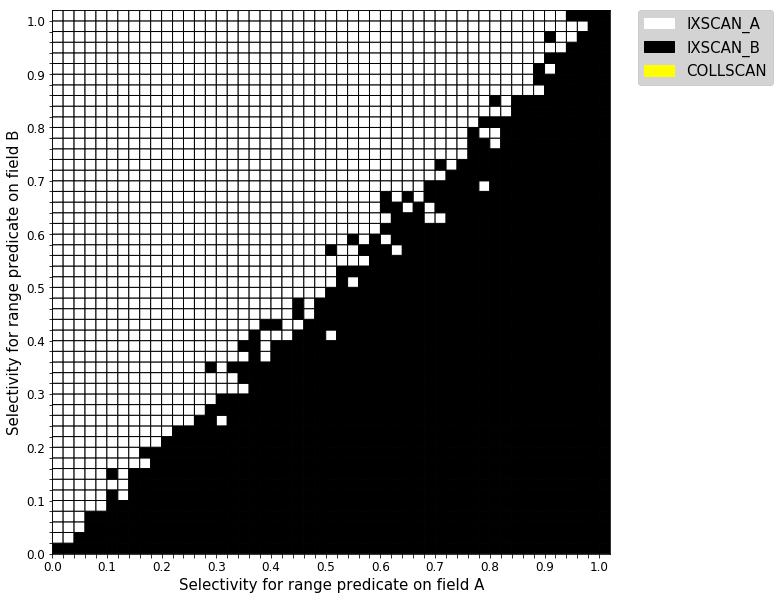
\includegraphics[width=\linewidth]{images/body/uniform_dist_practical_3095_10-23-2019_11_33_35.png}
%    \caption{A visualization of MongoDB V2 query plans}
%    \label{fig:linearv2}
%\end{figure}
%
%\begin{figure}[h]
%    \centering
%    \includegraphics[width=\linewidth]{images/body/uniform_dist_a%ctual_3095_10-23-2019_11_33_35.png}
%    \caption{A visualization of the optimal query plans}
%    \label{fig:linearreal}
%\end{figure}


%However, having high rate picking the sub-optimal 
%query plan does not necessary mean there will be 
%a huge performance drop. In other words, MongoDB 
%might still capable to provide a considerable 
%level of efficient query execution. Therefore, we
%are going to quantify the change in performance to 
%take a closer look at the impact of this issue. 


%\begin{figure}[h]
%    \centering
%    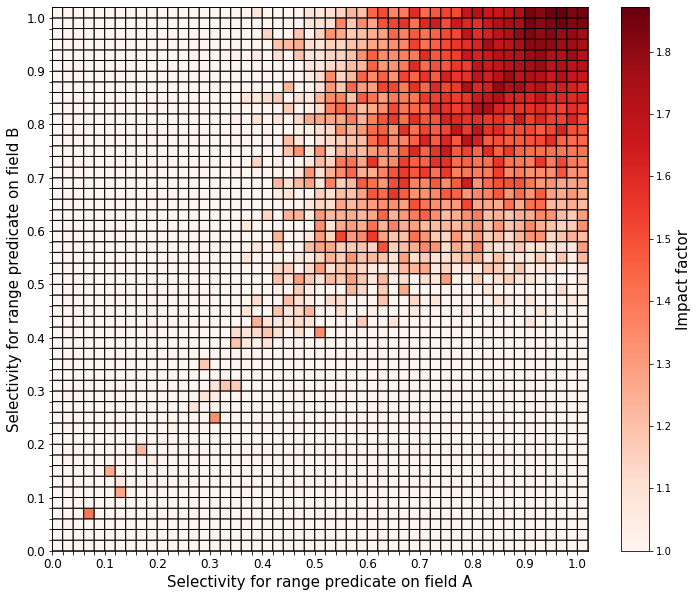
\includegraphics[width=0.9\linewidth]{images/body/uniform_dist_error_3095_11-09-2019_15_07_17.png}
%    \caption{A visualization of the impact of the preference bias issue}
%    \label{fig:diff1}
%\end{figure}

%In figure \ref{fig:diff1} we visualize the impact factor using the technique we explained in section \ref{sec:quant}. Different values of impact facto are mapped to distinct colours in the colour bar. Recall that the higher the impact factor is, the worse the chosen plan preforms. For example, an impact factor of 2 means the execution time of a chosen plan is twice the execution time of the optimal plan. And the value of 1 means the performance of the query plan is identical to the ideal baseline (i.e. the ideal case in which the optimal candidate has been chosen). Therefore, we can tell the dark red area in figure \ref{fig:diff1} indicates that the preference bias issue has a negative impact. The experimental results are in line with our expectations, as the selectivity of  both fields rises, the relative performance of the collection scan increases; as a result, the pixel colour gradually becomes darker along both axis. According to our measurement, the rate of an optimizal query plan been chosen is only 69.29\%. In the worst case, the preformance of the optimal plan is 86.83\% faster than MongoDB's choice. The overall performance of the query optimizer can be improved by 10.79\% if the \approachName approach is capable of choosing the optimal query plan. 




